\section{The Validation Process Case Study}

In this section we apply the concepts outlined in Sec.~\ref{sec:metrics} on a simplified example of the test method on an aggregator architecture similar to the one developed in previous work\cite{thavlov2013aggregation}. The sample aggregator name is  DTU-FlexServices, and it wants to sell ancillary services to the TSO called RisøGrid. The rest of this section presents the reference scenario, the example of the aggregator test and the evaluation process. 

\subsection{The aggregator architecture}
The objective of the DTU-FlexServices is to allocate a given amount of power over a controllable portfolio of resistive heating systems, each providing space heating to a detached household. The objective is subject to constraints on nominal power of the heating systems and indoor comfort, which is implemented as a tolerable band in which the temperature is allowed to vary given by the interval $\left[T_{min},T_{max}\right]$. It is assumed that feedback on indoor temperature is available to the aggregator, such that the aggregator in real-time can assess the available capacity of the controlled heating system and ensure that indoor constraints are not being violated in the future. Fig. \ref{fig:flow_diagram} presents the flow of data in the aggregator simulation framework. 
\begin{figure}[!t]
\centering
\includegraphics[width=\columnwidth]{pscc2016/flowchart.eps}
\caption{Flow diagram of the aggregator algorithm.}
\label{fig:flow_diagram}
\end{figure}
The aggregator uses a simple auto-regressive model with exogenous inputs (ARX) to assess the future available capacity of each individual households. The ARX model is given by,
\begin{equation}\label{eq:capacity}
  T_{i+1} - a\cdot T_i = b \cdot T_{a,i} + c \cdot \Phi_{s,i} + \boldsymbol{d}^T \boldsymbol{\Phi}_{h,i:i-\tau_{lag}}
\end{equation} 
where $T_i$ is the indoor temperature of the household at time step $i$, $T_a$ is the outdoor temperature, $\Phi_s$ is the solar irradiance and $\boldsymbol{\Phi}_{h,i:i-\tau_{lag}}$ is a vector with the most recent observed power consumptions, i.e. $\left[\Phi_{h,i},\Phi_{h,i-1} \cdots \Phi_{h,i-\tau_{lag}}\right]$. The lag parameter of the heat input, $\tau_{lag}\in\mathbb{N}_0$, is used to account for the potential time-lag that might exists between when heating is applied and when it is observed in the indoor temperature. $a$, $b$, $c\in\mathbb{R}$, and $\boldsymbol{d}\in\mathbb{R}^{\tau_{lag}+1}$ are the unknown parameters of the ARX model, which are found using prior data for power consumption of the heating system. For simplicity $\tau\equiv 0$ is assumed in the following. 

Each resistive heating system is assumed to be able to dispatch a continuous amount of power in the interval $\left[P_{min}, P_{max}\right]$, given by the nominal power of the heating system. Naturally, this is an approximation since heating systems in general will only be able to dispatch power in discrete steps due the composition of resistive loads. However, considering a portfolio of many entities, these discrete steps should level out and the assumption hold. 

To allocate the amount of power over the portfolio of resistive heating system, following unit commitment problem is formulated,
\begin{align}\label{eq:agg_dispatch}
  & \min\;\left|\; \sum_{j=1}^N \left(\Phi_{h,i,j}\right) - S_i \;\right|\; + \; \sum^{N}_{j=1}\Phi_{h,i,j}\mbox{W}\left(T_{i+1,j}\right)	\\[5mm]\nonumber
  & \mbox{s.t.} \quad P_{min,j} \leq \Phi_{h,i,j} \leq P_{max,j}  
\end{align}
where the decision variable  $\Phi_{h,i,j}\in\mathbb{R}$ is the amount of power being allocated to household $j$ at time step $i$, $N$ is the number of households in the portfolio, $S_i$ is the given set-point to the aggregator and $\mbox{W}\left(T_{i+1,j}\right)$ is a weight function of the predicted indoor temperature found from Equation \eqref{eq:capacity}. The weight function should be constructed such that $\mbox{W}\left(\cdot\right)<-1$ for $T_{i+1,j} < T_{min}$, thus making the last term dominate the cost function and force the allocated power up for household $j$. Likewise, $\mbox{W}\left(\cdot\right)>1$ for $T_{i+1,j} > T_{max}$, thus forcing the power down. Following linear weight-function is proposed,
\begin{equation}\label{eq:weight_fct}
  \mbox{W}\left(T_{i+1,j}\right) = \frac{2\left(T_{i+1,j}-T_{min,j} \right)}{T_{max,j} - T_{min,j}}-1 
\end{equation}
The aggregator framework, simulating the considered scenario, has been implemented in \textsc{matlab} and is presented in detail in previous work\cite{thavlov2013aggregation}.

\subsection{Reference Scenario}
The DTU-FlexServices aggregator wants to participate in the ancillary service markets with a FRR up-regulation service with a volume of 250 kW. The service will be provided through the flexibility in the heating of 100 houses with electric heaters which are distributed over a wide geographical area, i.e. they are not on the same feeder. Since it is the first time DTU-FlexServices participates in the market for this service, RisøGrid requires DTU-FlexServices to go through the validation process. Following the steps outlined in Sec.~\ref{sec:alignment}, the validation process consists of the following steps:
\begin{enumerate}
\item DTU-FlexServices presents the documentation for its portfolio.
\item RisøGrid is not risk averse and sets the test service requirements as:
    \begin{itemize}
        \item Response accuracy: maximum RMS error is equal to 50 kW
        \item The response should be sustained for one hour
    \end{itemize}
\item RisøGrid identifies the normal operation scenario as:
    \begin{itemize}
        \item The only source of uncertainty is the availability of the portfolio, which is a normal distribution between 70\% and 100\%. This also accounts for minor changes in the portfolio size.
    \end{itemize}
\end{enumerate}

In this paper we focus on a single source of uncertainty, therefore the test for time responsiveness, i.e. delay in the communications systems between the aggregator and a DER is not considered.

Having identified the relevant scenario, RisøGrid proceeds to carry out the simulation tests.

\subsection{Aggregator test}
Since the only source of uncertainty is a uniform distribution, the tests are carried out evenly across the 70\% - 100\% spectrum of availability. Samples of the simulation outcome can be seen in Fig.~\ref{fig:test100} and Fig.~\ref{fig:test70}.
\begin{figure}[!t]
%\centerline{
\centering
\subfloat[Response accuracy]{\includegraphics[width=0.85\columnwidth]{pscc2016/agg_power_ctrl_100SH_0STATIC_05PCT_REDUCTION.eps}%
\label{fig:ref100}}
%\vfill
\\
\subfloat[House Temperatures]{\includegraphics[width=\columnwidth]{pscc2016/agg_box_plot_100SH_0STATIC_05PCT_REDUCTION.eps}%
\label{fig:temp100}}%}
\caption{Simulation results of the 100\% availability test}
\label{fig:test100}
\end{figure}

\begin{figure}[!t]
%\centerline{
\centering
\subfloat[Response accuracy]{\includegraphics[width=0.85\columnwidth]{pscc2016/agg_power_ctrl_70SH_30STATIC_05PCT_REDUCTION.eps}%
\label{fig:ref70}}
%\vfill
\\
\subfloat[House Temperatures]{\includegraphics[width=\columnwidth]{pscc2016/agg_box_plot_70SH_30STATIC_05PCT_REDUCTION.eps}%
\label{fig:temp70}}%}
\caption{Simulation results of the 70\% availability test}
\label{fig:test70}
\end{figure}

The response accuracy of DTU-FlexServices and the average temperature of its portfolio can be seen in Fig.~\ref{fig:ref100} and Fig.~\ref{fig:ref70}. The distribution of the house temperatures can be seen in Fig.~\ref{fig:temp100} and Fig.~\ref{fig:temp70}, and it is clear that as the availability of the houses decreases, the temperature spread widens and the DTU-FlexServices is unable to track the FRR reference signal.

Having carried out the necessary test, RisøGrid proceeds to evaluate the results of the tests.

\subsection{Aggregator evaluation}
Since the case study looks at simplified setup, and the example does not take the time responsiveness metric into account, it does not make sense to use the aggregator performance metric mentioned in Sec.~\ref{sec:evaluation}. In this case, the root mean square (RMS) error is chosen to measure the response accuracy metric. The RMS is given by 
\begin{equation}
  \mbox{RMS} = \sqrt{\frac{1}{M}\sum_{i=1}^M\left(\sum_{j=1}^N\left(\Phi_{h,i,j}\right) - S_i\right)^2}
\end{equation}
where $\left[1,M\right]$ are the iterations where the aggregator has been activated. The results of the test are presented in Table~\ref{tab:results}. The average of the tests is below the requirement of maximum 50 kW. Therefore the DTU-FlexServices is certified to provide FRR up-regulation service to RisøGrid.

\begin{table}[!t]%% increase table row spacing, adjust to taste
\renewcommand{\arraystretch}{1.3}
% if using array.sty, it might be a good idea to tweak the value of
% \extrarowheight as needed to properly center the text within the cells
\caption{Performance of DTU-FlexServices}
\label{tab:results}
\centering
% Some packages, such as MDW tools, offer better commands for making tables
% than the plain LaTeX2e tabular which is used here.
\begin{tabular}{ll}
\toprule
Portfolio availability & RMS error\\
\midrule
100\% & 1.2784e-10\\
95\%  & 3.5724e-10\\
90\%  & 6.965e-10\\
85\%  & 25.9769\\
80\%  & 71.4127\\
75\%  & 83.018\\
70\%  & 93.9736\\
\midrule
Average & 39.1973\\
\bottomrule
\end{tabular}
\end{table}
